\documentclass{article}

\title{Gravity Lab}
\author{Henry Oehlrich \and Grace Jiang \and Ansh Aggrawal}

\usepackage{tikz}
\usepackage{capt-of}
\usepackage[labelfont=bf]{caption}
\usepackage[margin=1.25in]{geometry}
\usepackage{booktabs}
\usepackage{array}
\usepackage{siunitx}
\usepackage{amsmath}
\usepackage{csvsimple}

\newcolumntype{L}{>{$}l<{$}}

\begin{document}
\maketitle

\begin{figure}[ht]
    \begin{minipage}[b]{0.5\textwidth}
        \centering
        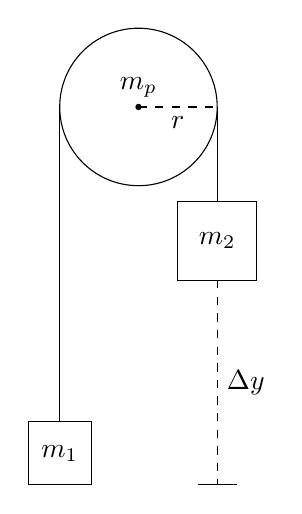
\begin{tikzpicture}
            \draw (0,5) node[above] {$m_p$} circle (1);
            \fill (0,5) circle (0.04);
            \draw[dashed] (0,5) -- (0.5, 5) node[below] {$r$} -- (1,5);

            \draw (1,5) -- (1,3.8);
            \draw (0.5,3.8) rectangle node {$m_2$} ++(1,-1);

            \draw (-1,5) -- (-1,1);
            \draw (-1.4,1) rectangle node {$m_1$} ++(0.8,-0.8);

            \draw[dashed] (1,2.8) -- (1,1.5) node[right] {$\Delta y$} -- (1,0.2);
            \draw (0.75,0.2) -- (1.25,0.2);
        \end{tikzpicture}
        \caption{Lab setup}
        \label{fig:setup}
    \end{minipage}%
    \begin{minipage}[b]{0.5\textwidth}
        \centering
        \begin{tabular}{l|l}
            \toprule
            Symbol & Value \\
            \midrule
            $\Delta y$ & \qty{1.67}{\meter} \\
            $m_1$ & \qty{0.01}{\kilogram} \\
            $g$ & \qty{9.81}{\meter\per\second\squared} \\
            $m_p$ & \qty{0.05}{\kilogram} \\
            $r$ & \qty{0.05}{\meter} \\
            $m_2$ & varied \\
            $t$ & measured \\
        \end{tabular}
        \captionof{table}{Constants and Variables}
    \end{minipage}
\end{figure}

\begin{equation}
    F_s = g(m_2 - m_1)
\end{equation}

\begin{figure}[ht]
    \begin{minipage}[b]{0.5\textwidth}
        \centering
        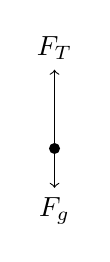
\begin{tikzpicture}
            \fill (0,0) circle (0.07);
            \draw[->] (0,0) -- (0,-0.5) node[below] {$F_g$};
            \draw[->] (0,0) -- (0,1) node[above] {$F_T$};
        \end{tikzpicture}
        \caption{Free body diagram of $m_1$}
        \label{fig:fbd1}
    \end{minipage}%
    \begin{minipage}[b]{0.5\textwidth}
        \centering
        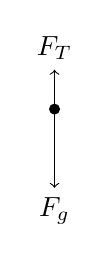
\begin{tikzpicture}
            \fill (0,0) circle (0.07);
            \draw[->] (0,0) -- (0,-1) node[below] {$F_g$};
            \draw[->] (0,0) -- (0,0.5) node[above] {$F_T$};
        \end{tikzpicture}
        \caption{Free body diagram of $m_2$}
        \label{fig:fbd2}
    \end{minipage}%
\end{figure}

\begin{figure}[ht]
    \centering
    \begin{tabular}{l|l|l|l}
        \toprule
        $m_2$ (\si{\kilogram}) & time (\si{\second}) & $m_2 - m_1$ (\si{\kilogram}) & $F_s$ (\si{\newton}) \\
        \midrule
        0.02 & 1.461 & 0.01 & 0.0469 \\
        0.02 & 1.441 & 0.01 & 0.0483 \\
        0.02 & 1.228 & 0.01 & 0.0664 \\
        0.02 & 1.195 & 0.01 & 0.0702 \\
        0.02 & 1.276 & 0.01 & 0.0615 \\
        0.02 & 1.290 & 0.01 & 0.0602 \\
        0.02 & 1.860 & 0.01 & 0.029 \\
        0.03 & 0.936 & 0.02 & 0.153 \\
        0.03 & 1.016 & 0.02 & 0.129 \\
        0.03 & 0.949 & 0.02 & 0.148 \\
        0.03 & 1.009 & 0.02 & 0.131 \\
        0.03 & 1.006 & 0.02 & 0.132 \\
        0.03 & 0.931 & 0.02 & 0.154 \\
        0.03 & 1.000 & 0.02 & 0.134 \\
        0.10 & 0.667 & 0.09 & 0.826 \\
        0.10 & 0.683 & 0.09 & 0.788 \\
        0.10 & 0.669 & 0.09 & 0.821 \\
        0.10 & 0.686 & 0.09 & 0.781 \\
        0.10 & 0.691 & 0.09 & 0.770 \\
        0.04 & 0.896 & 0.03 & 0.208 \\
        0.04 & 0.823 & 0.03 & 0.247 \\
        0.04 & 0.801 & 0.03 & 0.260 \\
        0.04 & 0.897 & 0.03 & 0.208 \\
        0.04 & 0.834 & 0.03 & 0.240 \\
        0.04 & 0.887 & 0.03 & 0.212 \\
        0.04 & 0.889 & 0.03 & 0.207 \\
    \end{tabular}
    \caption{Data}
    \label{fig:data}
\end{figure}

\end{document}
